\documentclass{beamer}

\mode<presentation>
{
  %\usetheme{AnnArbor}
  %\usetheme{Montpellier}
  %\usetheme{Hannover}
  %\usetheme{Singapore}
  \usetheme{Madrid}
}

\newcommand*\oldmacro{}
\let\oldmacro\insertshorttitle% ursprüngliche Definition sichern
\renewcommand*\insertshorttitle{%
  \oldmacro
  \hfill\insertframenumber\,/\,\inserttotalframenumber}

\setbeamertemplate{navigation symbols}{}

\usepackage[english]{babel}
\usepackage{hyperref}

%\usepackage[latin1]{inputenc}
\usepackage[utf8]{inputenc}

%\usepackage{hyperref}

% WTF? times? serious?
%\usepackage{times}
\usepackage[T1]{fontenc}

\usepackage{listings}

%\usepackage{tabularx}

\title[Project Presentation]{Data and Information Visualization \\ MMO CombatLog Visualization}

%\subtitle {Untertitel} (optional)

\author[Brauer, Fortmann, Schmauder]
{S. Brauer \and M. Fortmann \and F. Schmauder}

\institute[UPB]{Institute for Computer Science}

\date{July 5, 2012}


\subject{Computer Science}

\pgfdeclareimage[height=0.5cm]{university-logo}{upb_logo.png}
\logo{\pgfuseimage{university-logo}}



% Folgendes sollte gelöscht werden, wenn man nicht am Anfang jedes
% Unterabschnitts die Gliederung nochmal sehen möchte.
%\AtBeginSubsection[]
%{
%  \begin{frame}<beamer>{Gliederung}
%    \tableofcontents[currentsection,currentsubsection]
%  \end{frame}
%}



\begin{document}

\begin{frame}
  \titlepage
\end{frame}

\begin{frame}{Visualization Goals}
\begin{itemize}
	\item Achieve Motivation by allowing players to compare their performance with other players 
	\item Improve Performance by enabling a detailed break down into components making it possible to find flaws in playstyle
	\item As the group leader: watch a players performance over time and decide to keep him/her in the group or not (e.g. if the players performance is decreasing)
\end{itemize}
\end{frame}

\begin{frame}{Data Model}
\begin{itemize}
	\item The Data consists of a nominal and a quantitative part
	\item Timestamp for each data point categorizing it as reliable, non-continous time-series data
	\item Each data point has a nominal part (player and spell assocation)...
	\item ... and a quantitative part (Amount of actual damage/healing done)
\end{itemize}
\end{frame}

\begin{frame}{Potential Users}
\begin{itemize}
	\item Gamers!
	\item More Specific: 
	\begin{itemize}
		\item Gamers playing the same game
		\item Group members/leader analysing their performance
		\item Players from other groups working on the same encounter looking for ideas
	\end{itemize}
\end{itemize}
\end{frame}


\begin{frame}{Visualization Techniques}
\begin{itemize}
	\item Line Graphs for visualization over time
	\item Pie Chart for visualization of ratios
\end{itemize}
	\begin{figure}
		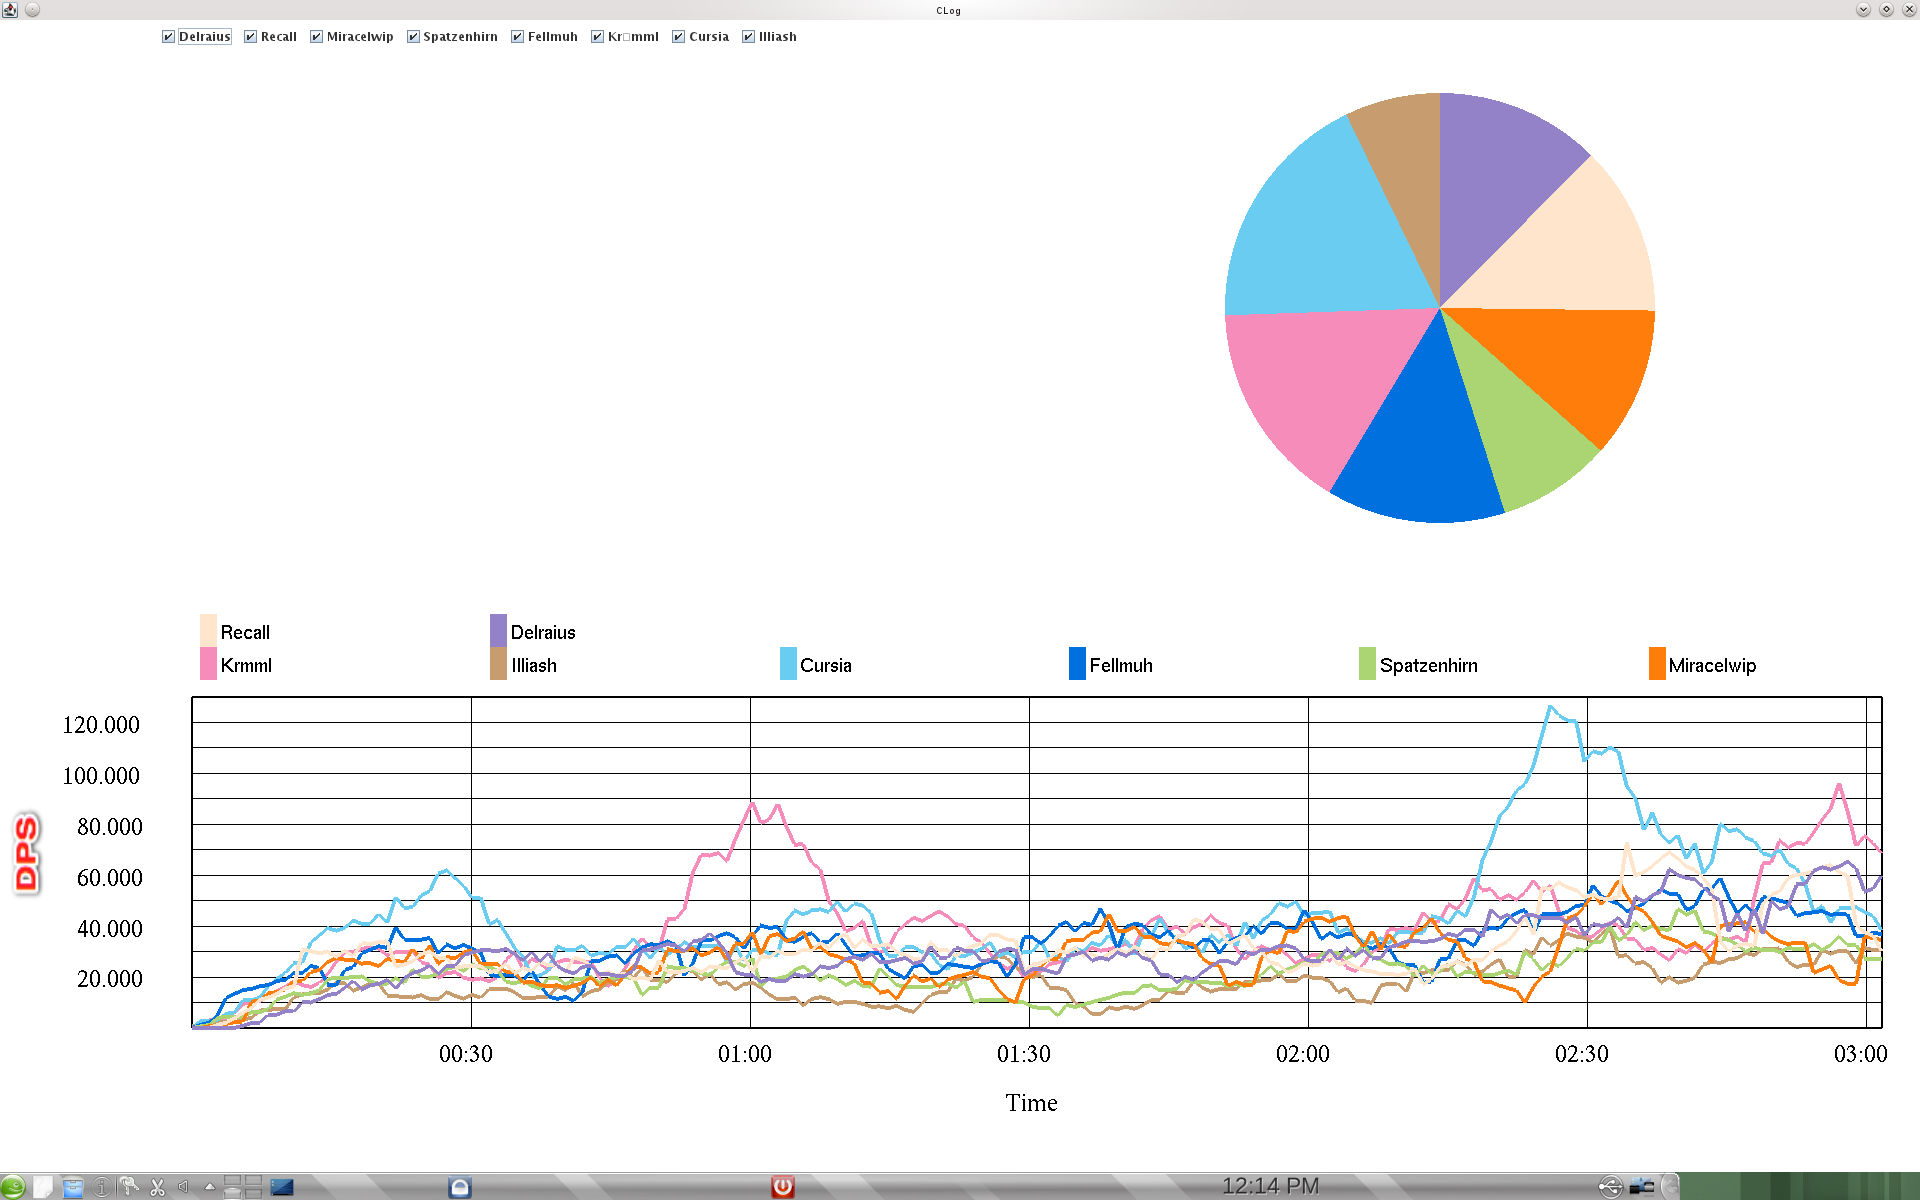
\includegraphics[width=\textwidth]{viz.png}
	\end{figure}
\end{frame}

\begin{frame}{Interaction Techniques}
\begin{itemize}
	\item Tooltips conserving detailed information
\end{itemize}
	\begin{figure}
		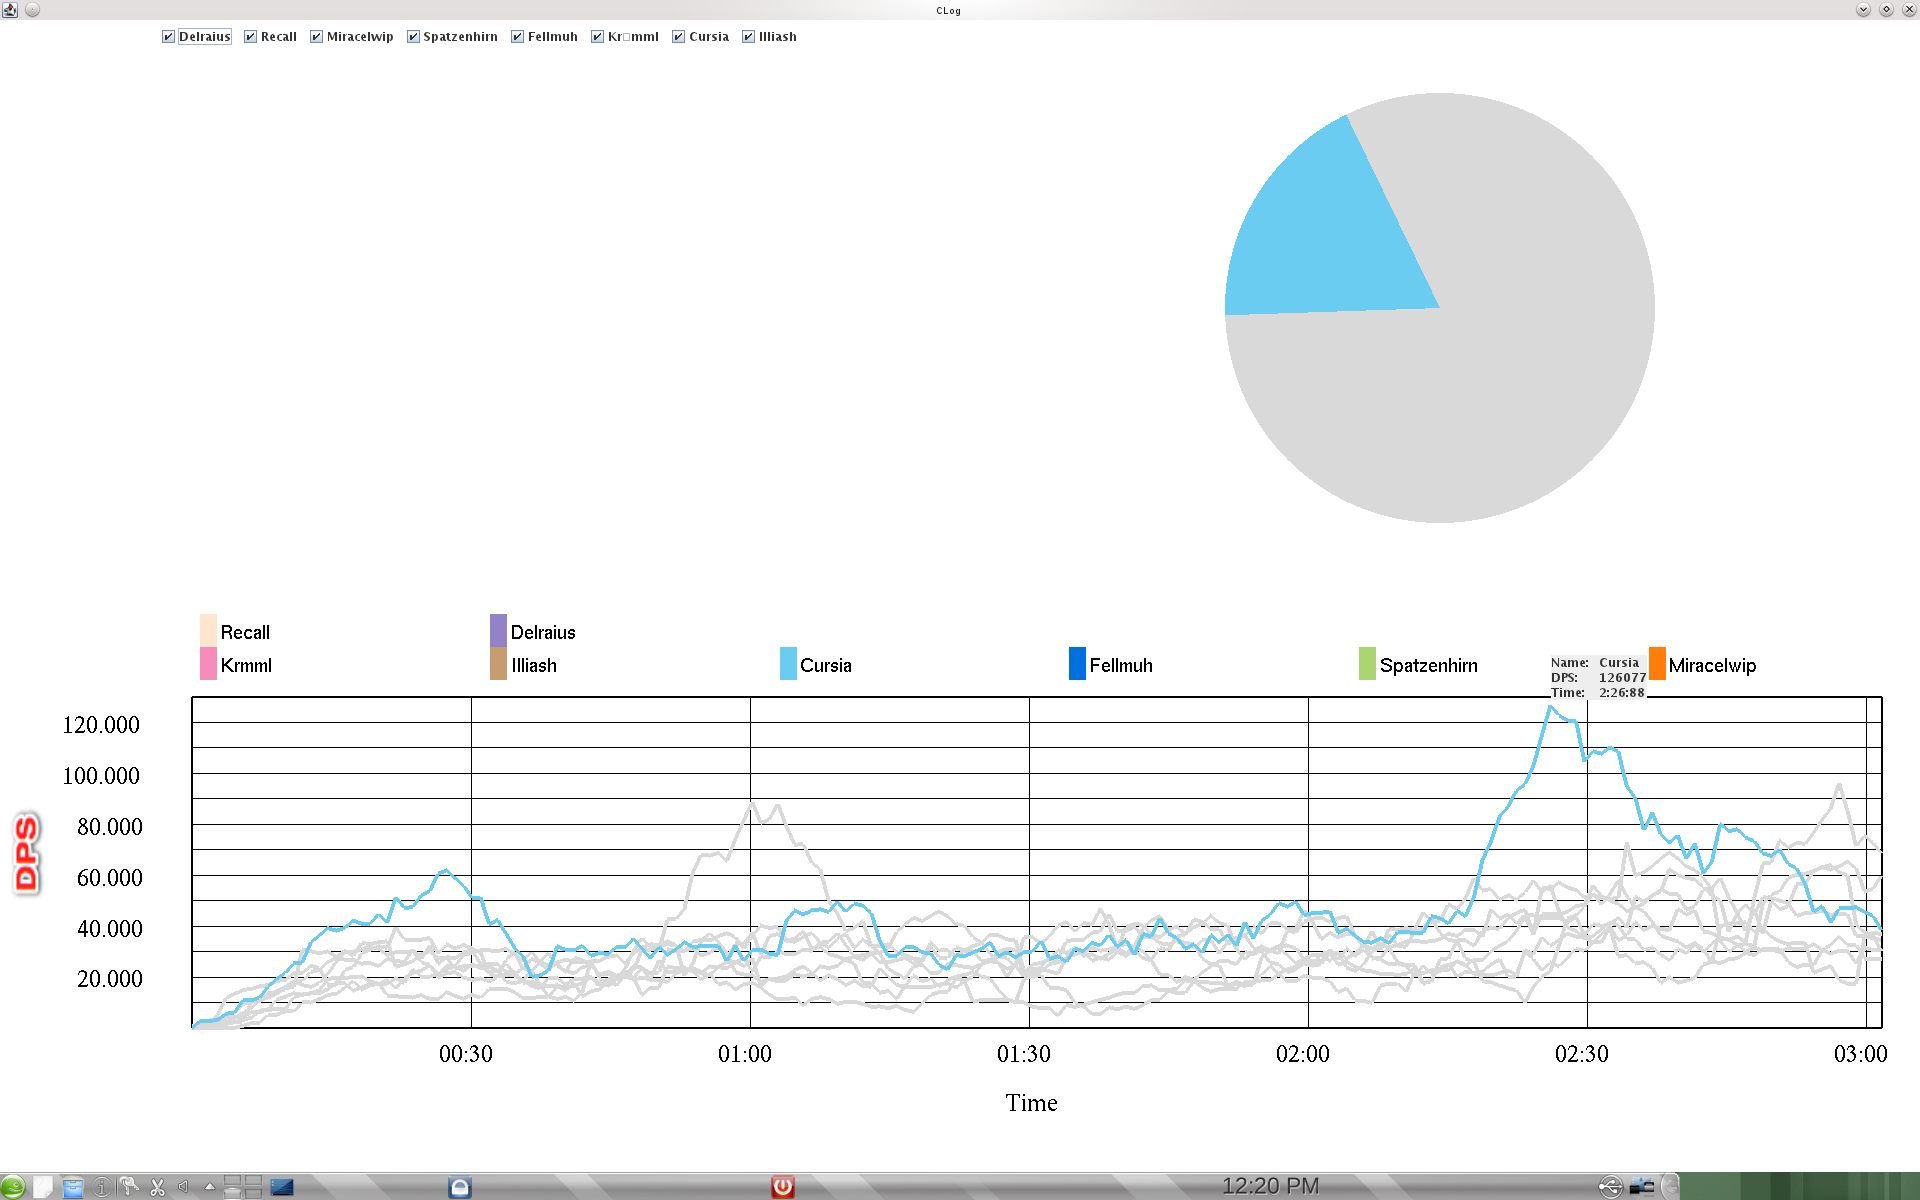
\includegraphics[width=\textwidth]{tooltip.png}
	\end{figure}
\end{frame}

\begin{frame}{Interaction Techniques cont.}
\begin{itemize}
	\item Selective Filtering to increase overview
\end{itemize}
	\begin{figure}
		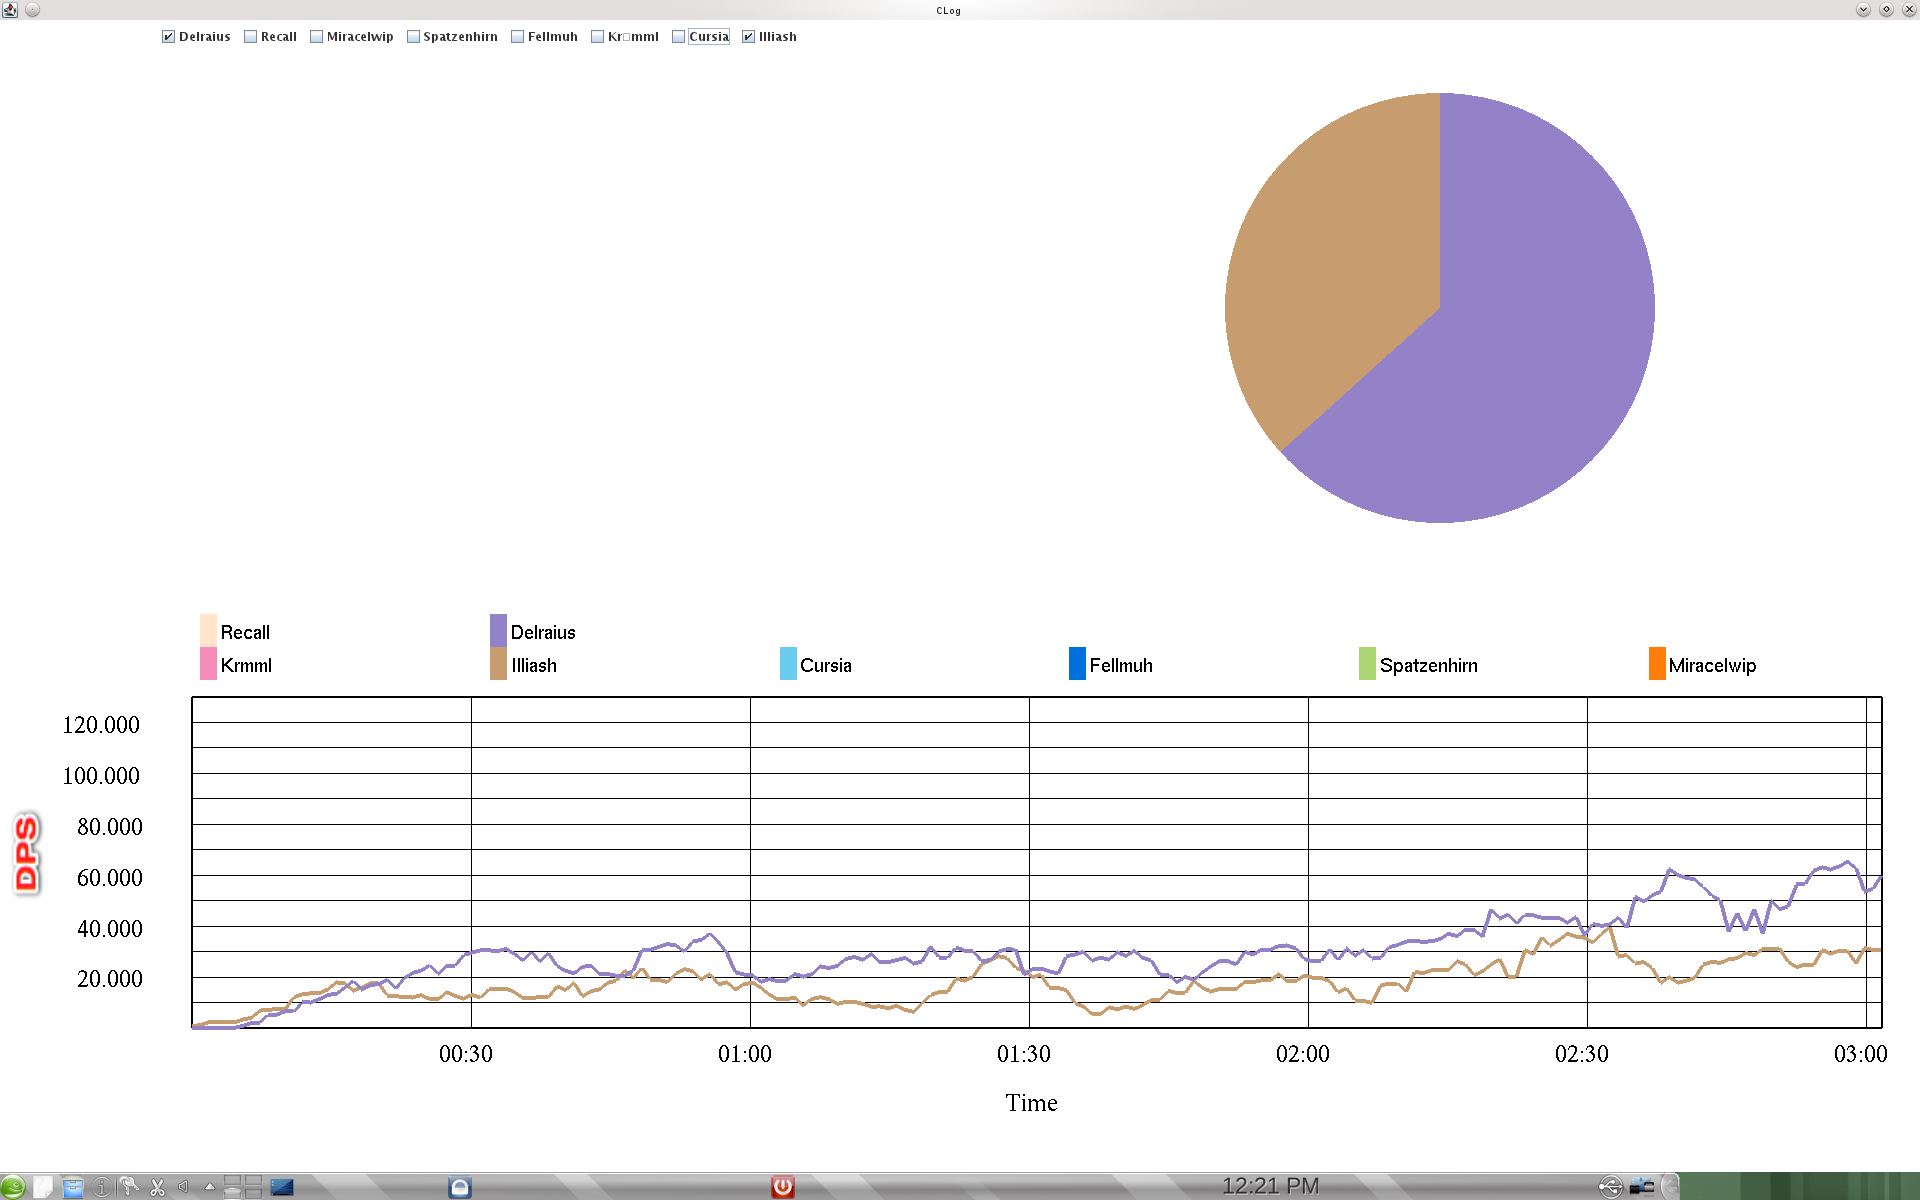
\includegraphics[width=\textwidth]{filter.png}
	\end{figure}
\end{frame}

\begin{frame}{Interaction Techniques cont.}
\begin{itemize}
	\item Select and Zoom (Click) for data break down
\end{itemize}
	\begin{figure}
		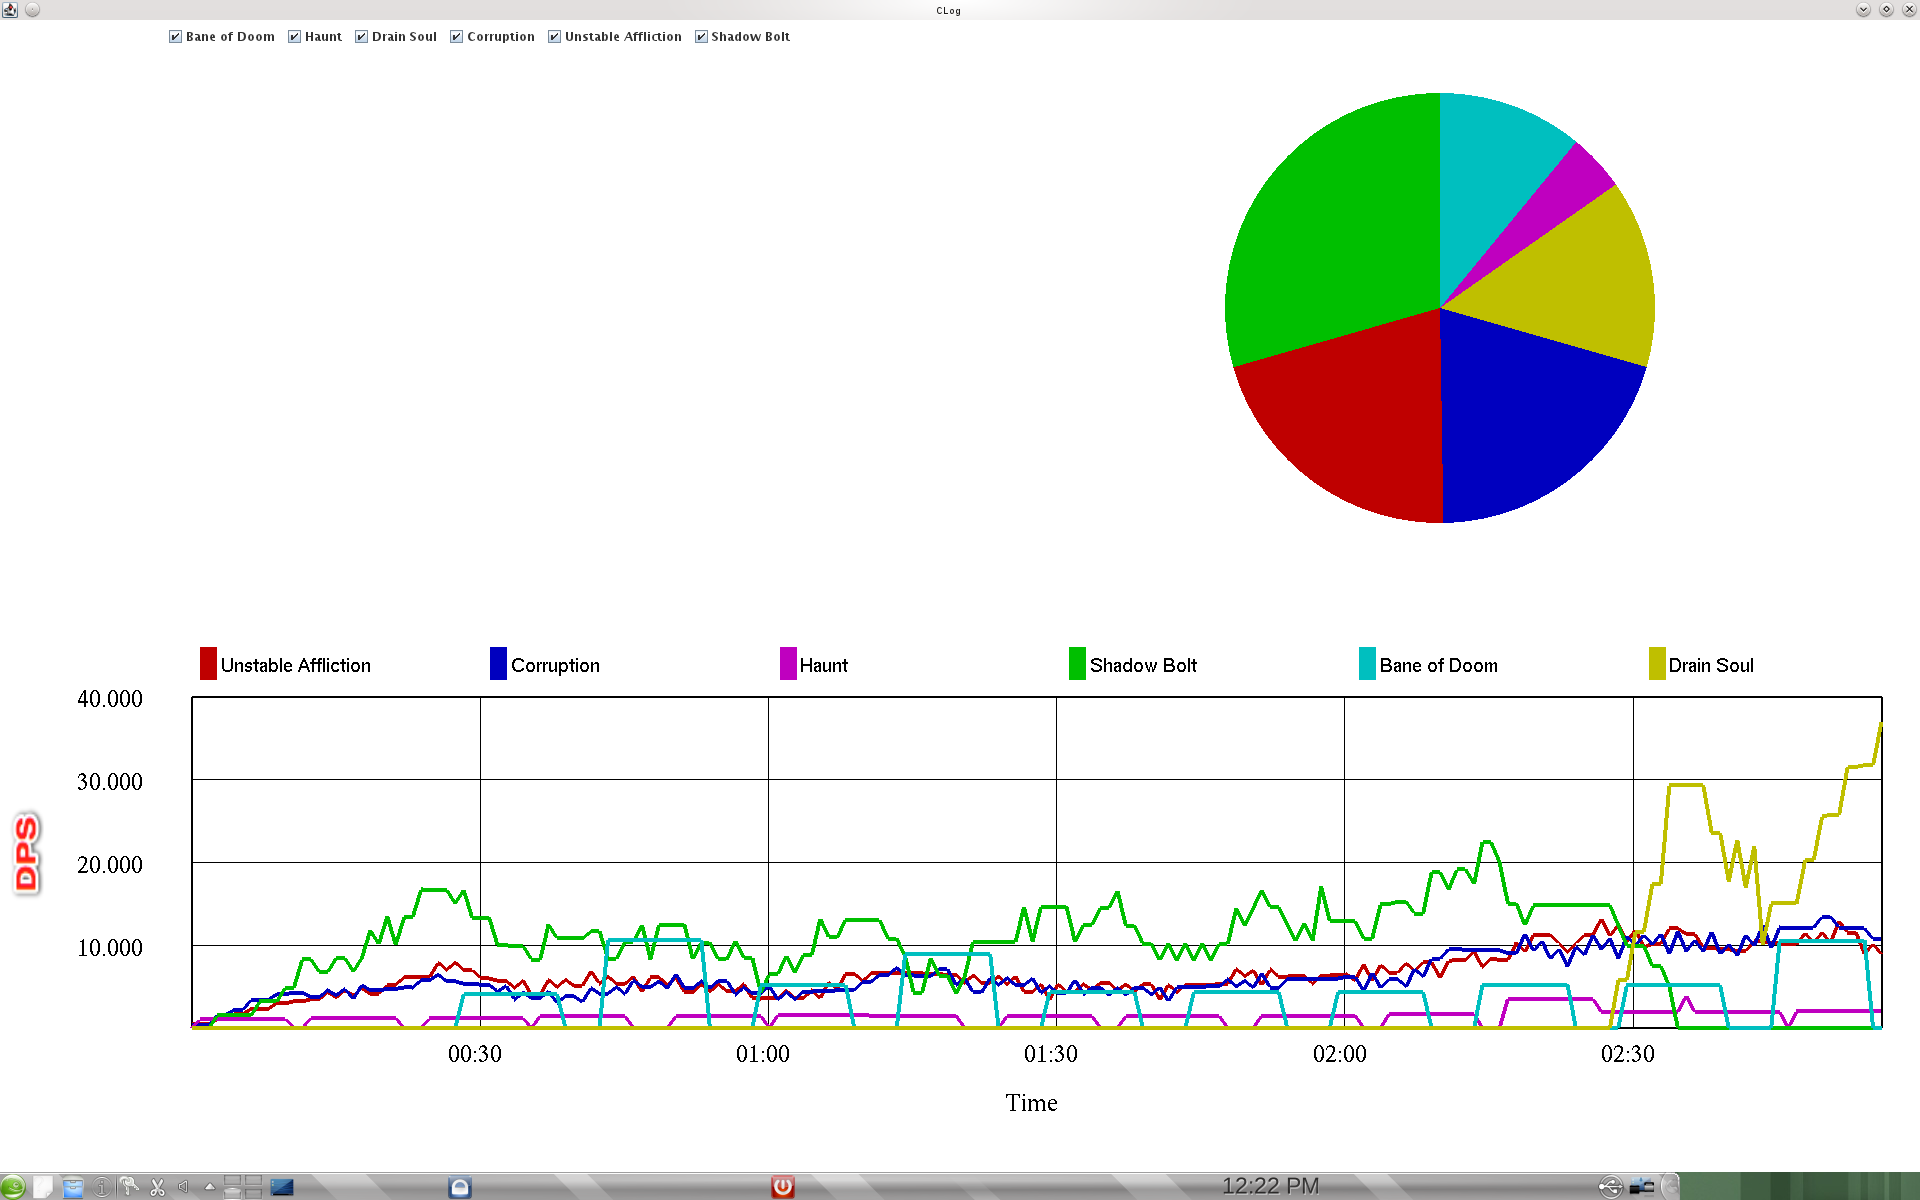
\includegraphics[width=\textwidth]{detail.png}
	\end{figure}
\end{frame}

\begin{frame}{Interaction Techniques cont.}
\begin{itemize}
	\item Select and Zoom (Time Shift) to select a specific time window
\end{itemize}
	\begin{figure}
		
\includegraphics[width=\textwidth]{time.png}
	\end{figure}
\end{frame}

\begin{frame}{Usefulness for the Vis. goals}
\begin{itemize}
	\item We exercised user tests as usability evaluation
	\item Testpersons were gamers as well (tool has no use for people not knowing the game)
	\item Testpersons told us that apart from the usability evaluation the tool was very useful for analysis
	\item Webservices providing similar functionality and techniques are widely used in the gaming scene
\end{itemize}
\end{frame}

\begin{frame}{Technical Solutions}
\begin{itemize}
	\item Preprocessing heavily used because of huge data amount
	\item Simple line-wise String Parser
	\item Only basic OpenGl commands
	\item HashMaps used for almost everything
	\item "TimeBuffer" provides a small wrapper around queues and is used for DPS(Damage per Second) calculation
\end{itemize}
\end{frame}

\begin{frame}{Anything else}
\begin{itemize}
	\item Commands:
	\begin{itemize}
		\item Left Click for spell break down (either on line of pie)
		\item Right Click to go one level up from spell break down
		\item Middle Mouse Click to switch between two data sets
		\item Left/Right Arrow key to Decrease/Increase Starttime (Time Shift)
		\item Top/Down Arrow key to Increase/Decrease Endtime (Time Shift)
	\end{itemize}
\end{itemize}
\end{frame}

\begin{frame}{References}
\begin{itemize}
	\item Class Color Conventions: \url{http://www.wowwiki.com/Class_colors}
	\item CombatLog Line Elements: \url{http://www.wowwiki.com/API_COMBAT_LOG_EVENT}
\end{itemize}
\end{frame}

\end{document}

